\documentclass[11pt,a4paper]{article}
\usepackage[T1]{fontenc}
\usepackage{lmodern,amsmath,amssymb,booktabs,microtype,graphicx}
\usepackage[margin=24mm]{geometry}
\usepackage[colorlinks=true,urlcolor=blue,linkcolor=blue]{hyperref}
\newcommand{\Js}{\mathcal J_s}
\newcommand{\Rh}{\widehat R}
\newcommand{\av}[1]{\tau\!\left(#1\right)}
\DeclareMathOperator{\sech}{sech}
\title{An ordering-odd composite channel\\Mixed singlet growth, propagation, and a cubic vertex}
\author{Alan Day \and Chengheng\thanks{AI research assistant (OpenAI).}}
\date{Local research note --- 6 November 2026}
\begin{document}\maketitle
\begin{abstract}
We apply the existing unequal-species semiclassical four-point function
to the quadratic and cubic derivative singlets. This fixes the entire
leading fixed-time mixed commutator, rather than just its Taylor series.
The equal-time commutator also gives a normalized ordering-odd composite
with the exact $q^5$ two-energy kernel. Its product decomposition, a
three-time cubic vertex, and a nonzero fourth-moment excess distinguish
this composite from an independent Gaussian probe. These are explicit
instances of the extra commutator primaries identified by Lin--Stanford.
\end{abstract}
\section{A closed interaction coefficient and its state}
Use standard CAR, complex Gaussian number-preserving $p$-body $H_s$
including overlapping index sets, and the annealed normalized trace
$\tau$ at $\beta=\mu_{\rm chem}=0$. Set $\hbar=1$ and take
\[
 N,p\to\infty,\quad\lambda=p^2/N>0,\quad h=4\lambda,\quad q=e^{-h},
 \quad H_{\rm src}=H_s/(2\Js),\quad \tau H_{\rm src}^2=h^{-1}.
\]
The preceding note \cite{local} constructed normalized Hermitian
singlets $X,\Rh$ with joint multiprobe weights $d_X=2,d_{\Rh}=3$.
Time below is string time, $u=2\Js t$, and small $\lambda$ is taken
after DS. The sourced fixed-time expansion \cite{LS,Streicher} yields
\begin{equation}
 \boxed{D_{23}(t):=\av{[X(t),\Rh]^\dagger[X(t),\Rh]}
       =48\lambda\cosh(4\Js t)+O(\lambda^2).}\label{growth}
\end{equation}
The remainder denotes the semiclassical asymptotic expansion at fixed
times, not a uniform numerical bound at scrambling times.

At every fixed $q<1$ in DS, define two unit-norm Hermitian composites
\begin{equation}
 K=\frac{-i[X,\Rh]}{\sqrt{2(1-q^6)}},\qquad
 S=\frac{\{X,\Rh\}}{\sqrt{2(1+q^6)}}.\label{KS}
\end{equation}
Their exact product decomposition is
\begin{equation}
 X\Rh=\sqrt{\frac{1+q^6}{2}}S+i\sqrt{\frac{1-q^6}{2}}K,\qquad
 \tau(SK)=0.\label{product}
\end{equation}
The ordering-odd squared component is $(1-q^6)/2=12\lambda+O(\lambda^2)$.
It is small but dynamically measurable. It is not being identified with
a physical scattering probability without a bulk state map.

\newpage
\section{From the sourced four-point function to a covariance}
For general distinct probe labels $d,e$, write
$g_d(x)=\sech^{2d}x$. Lin--Stanford Eq.~(205), with their deformation
parameter replaced by $h$ and their thermal parameter $c\to1$, gives
the crossed connected coefficient
\begin{equation}
 \frac{\av{V_1W_2V_3W_4}-G_{d,h}(u_1-u_3)G_{e,h}(u_2-u_4)}h
 \longrightarrow
 -de\,g_d(x)g_e(y)\frac{\cosh A}{\cosh x\cosh y},\label{cross}
\end{equation}
where $x=u_1-u_3$, $y=u_2-u_4$, $A=u_1+u_3-u_2-u_4$.
Here the subtracted two-point functions are the full finite-$h$ ones.
The continuation is $\tau_+=-ix$, $\tau_+'=-iy$, $\tau_-=iA$.
The mutual crossing factor is already included in this connected
coefficient; it must not be multiplied in a second time.

The uncrossed formula follows from the energy-exchange term in
Lin--Stanford Appendix G.2, Eq.~(388):
\begin{equation}
 \av{V_1V_3W_2W_4}_{c}/h
 \longrightarrow -de\,g_d(x)g_e(y)\tanh x\tanh y.\label{uncross}
\end{equation}
The orientation of each pair matters. For the orderings in a product of
commutators, one of the two separations reverses. Expanding the four
terms and canceling their full disconnected parts gives, for
$B_h(u,v)=-i[V(u),W(v)]/\sqrt h$,
\begin{align}
 \lim_{h\to0}\av{B_h(u,v)B_h(u',v')}
 &=2de\,\sech^{2d+1}(u-u')\sech^{2e+1}(v-v')\notag\\
 &\quad\times\left[\cosh(u+u'-v-v')
              +\sinh(u-u')\sinh(v-v')\right].\label{cov}
\end{align}
On the diagonal $(u',v')=(u,v)$ this is $2de\cosh(2(u-v))$.
With $d=2,e=3$, $h=4\lambda$, it proves the coefficient in
Eq.~\eqref{growth}. On the simultaneous-time line $u=v$, $u'=v'$,
the covariance reduces to $12\sech^{10}(u-u')$.

This covariance is an application of the established four-point
formula. The relation to commutator-created states is already explicit
in Lin--Stanford Section~4.8 and Appendix~F.1 \cite{LS}. We retain
their interpretation as extra ordering channels and determine the
concrete $d=2,3$ operator and its finite-$q$ observables below.

\paragraph{Independent local check.}
Direct mixed Wick enumeration on four distinct time rays through
degree eight reproduces all 20 coefficients of \eqref{cov}. It also
checks 60 cancellations of nonpositive Laurent powers of $h$.
This checks signs, orientations, and normalization; the full-time
formula is obtained from the sourced expansion, not inferred from
these finitely many coefficients.

\newpage
\section{Exact propagation and the three-time vertex}
The two ordered product states $X\Rh$ and $\Rh X$ have Gram matrix
\begin{equation}
 \begin{pmatrix}1&q^6\\q^6&1\end{pmatrix}.
\end{equation}
They are zero-Hamiltonian-chord seeds with total label $2+3=5$.
Their even and odd combinations give \eqref{KS}; this is precisely the
$k=0$ case of the normalized ordering combinations in Lin--Stanford
Eqs.~(110),(368). For this case the normalization is immediate, without
any all-$k$ overlap ansatz.

Insert any two strings of Hamiltonians between two composite blocks.
No Hamiltonian endpoint lies inside a block. A Hamiltonian chord
therefore crosses both constituent matter chords or neither, independent
of the order inside the block. Switching that order changes only the
mutual factor $q^6$. Summing the two orders yields, for all fixed
nonnegative integers $a,b$,
\begin{equation}
 \av{K H_s^a K H_s^b}=\av{S H_s^a S H_s^b}
 =\sigma^{a+b}P_{ab}(q,q^5),\qquad
 \av{K H_s^a S H_s^b}=0,\label{all}
\end{equation}
where $\sigma^2=\Js^2/\lambda$ and $P_{ab}$ is the established
unit-variance single-probe chord moment. Compact moment determinacy
gives the full Mehler two-energy measure $d\nu_{KK}=d\nu_{SS}=d\mu_{q^5}$,
$d\nu_{KS}=0$. In particular,
\begin{equation}
 \av{K(t)K}=G_{q^5}(t)\longrightarrow\sech^{10}(2\Js t).
\end{equation}
This identifies two equivalent propagation representations; it does
not identify their multiplication laws.

There is also an exact vertex. In a three-time word the first composite
block has adjacent $X,\Rh$ endpoints. Exchanging them changes only the
single mutual matter crossing, even with arbitrary Hamiltonian powers
on the three external arcs. Consequently
\begin{align}
 \av{K(t_0)X(t_1)\Rh(t_2)}
 &=i\sqrt{\frac{1-q^6}{2}}\,
   \av{\Rh(t_0)X(t_0)X(t_1)\Rh(t_2)}.\label{vertex}
\end{align}
The right side is the known uncrossed four-point function. At fixed
times its leading term is therefore
\begin{equation}
 \boxed{\av{K(t_0)X(t_1)\Rh(t_2)}
 =i\sqrt{12\lambda}\,g_2(u_0-u_1)g_3(u_0-u_2)
      +O(\lambda^{3/2}).}\label{cubic}
\end{equation}
At equal times this vertex is exactly $i\sqrt{(1-q^6)/2}$; reversing
the order of $X,\Rh$ changes its sign. The imaginary value is consistent
with a trace of three noncommuting Hermitian operators.

\newpage
\section{Higher points distinguish the composite channel}
Exact enumeration of the eight constituent insertions gives
\begin{equation}
 \boxed{\av{K^4}=2+q^{25}
       +\frac{(1-q^6)^2}{2}(1+q^4+q^9).}\label{fourth}
\end{equation}
The first two terms would be the fourth moment of an independent
$d=5$ probe. The extra term is strictly positive for $0<q<1$, and
is $54h^2+O(h^3)=864\lambda^2+O(\lambda^3)$. Thus even an exact
$q^5$ two-point kernel is insufficient to promote $K$ to an independent
probe species. Its nonzero cubic vertex already displays the connection
to its two constituents at order $\sqrt\lambda$.

As further fixed-moment checks, $\tau K^2=1$, $\tau K^4\to3$, and
$\tau K^6\to15$ as $q\to1$. These values alone do not prove a joint
Gaussian limit including the rescaled commutator. The full finite-$q$
sixth-moment polynomial is retained in the calculation record.

\paragraph{A concrete place in the two-matter space.}
The ordering-odd seed is an additional copy of the label-five chord
primary. Its unnormalized norm vanishes as $\sqrt{12h}$, but the
normalized state in \eqref{KS} survives. Applying the existing
fixed-descendant contraction from the earlier local notes \cite{local}
to this unit seed gives the positive discrete-series module $D^+_5$:
\[
 K_+e_n=\sqrt{(n+1)(10+n)}\,e_{n+1},\quad
 K_-e_n=\sqrt{n(9+n)}\,e_{n-1}.
\]
Here $K_\pm$ are chord generators, distinct from the composite $K$.
The same two-sided positive generator $Q_h=\bar n+\Pi_h$ applies.
Its limiting seed measure is the already established gamma law
\begin{equation}
 d\nu_Q(p)=\frac{2^{10}}{\Gamma(10)}p^9e^{-2p}\,dp,
 \qquad \av{e^{-isQ}}_K=(1+is/2)^{-10}.\label{Q}
\end{equation}
This is an application of the previous norm-controlled representation
construction. It does not require assigning a new physical mass to
the label five.

\paragraph{Interaction interpretation.}
Equation \eqref{product} resolves the change of product order into a
specific orthogonal state, while \eqref{vertex} fixes its overlap with
the constituent pair. This is more information than the growth rate
alone. The next bulk construction should preserve both this channel and
the ordinary product channel, and reproduce the vertex and propagation
simultaneously. A model with independent commuting fields and no extra
ordering sector would miss the leading mixed commutator.

\newpage
\section{Finite-deformation evidence}
\begin{center}
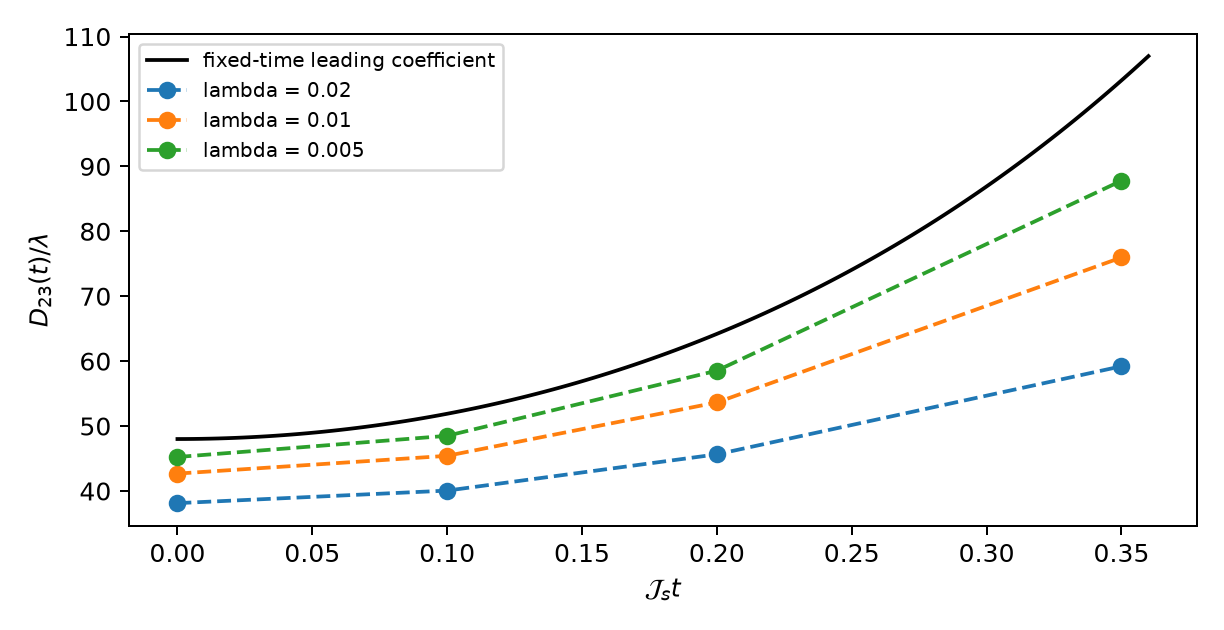
\includegraphics[width=.95\linewidth]{../../results/susskind-commutator-primary/mixed-growth.png}
\end{center}
\noindent The exact BINT kernel \cite{BINT}, with the restored $q^6$
factor, approaches the fixed-time coefficient as $\lambda$ decreases.
The plot retains the finite-deformation discrepancies. With $\Js=1$,
the smallest computed value $\lambda=.005$ gives
\begin{center}
\begin{tabular}{rrrr}
\toprule
$t$&$D_{23}(t)/\lambda$&$48\cosh(4t)$&relative difference\\\midrule
0&45.231825&48.000000&$-5.77\%$\\
.10&48.493930&51.891474&$-6.55\%$\\
.20&58.530332&64.196877&$-8.83\%$\\
.35&87.789905&103.243126&$-14.97\%$\\\bottomrule
\end{tabular}
\end{center}
The Richardson estimate from $\lambda=.01$ and $.005$ has relative
differences $-0.44\%$, $-0.61\%$, $-1.20\%$, and $-3.52\%$, respectively.
It is a diagnostic extrapolation, not an error certificate.

For $\lambda=.02,.01,.005$, the Jacobi sizes are $244,497,1032$.
Each includes an analytic vacuum/source Taylor-tail bound from the
preceding mixed-kernel construction, valid for $|t|\le.35$ in exact
arithmetic. Enlarging each cutoff by 16 changes the selected $t=.35$
OTOC by at most $2.78\,10^{-15}$.

Four additional checks evaluate the original nonsymmetric BINT index
sum at 50 decimal digits, at the same finite size $L=18$. The maximum
absolute difference from the symmetric positive formula is
$1.97\,10^{-17}$, with relative difference below $5.94\,10^{-15}$.
The nonsymmetric summation condition number stays below $1.000004$;
the subtraction condition number of $D_{23}=2(1-F_{23})$ in the main
scan is at most $16.69$. Full values, relative errors, and tail bounds
are saved, rather than interpreting cutoff stability as asymptotic accuracy.

\newpage
\appendix
\section{Evidence, scope, and next step}
The exact checks use independent integer crossing enumeration in the
already established joint $(H_s,X,\Rh)$ law:
\begin{itemize}
\item 25 two-arc moments through eight external Hamiltonians verify
      the $q^5$ propagation and the vanishing $K$--$S$ cross measure.
\item 50 three-arc identities through six external Hamiltonians
      verify the exact exchange factor in \eqref{vertex}.
\item The normalized moments of $K$ of orders two, four, and six are
      computed before taking limits, including the positive excess in
      \eqref{fourth}.
\item Four distinct time rays through degree eight verify 20 covariance
      coefficients and 60 Laurent cancellations in \eqref{cov}.
\end{itemize}
The arbitrary-degree two-arc and three-arc statements are proved by
the endpoint-exchange arguments on page~3. The finite checks verify
those arguments' algebraic implementation. Fixed-$q$ real-time
continuation uses the bounded limiting chord model; finite-$N$ moment
convergence and Taylor/H\"older control were established in the preceding
mixed-singlet note. The small-$h$ real-time coefficients use the sourced
semiclassical expansion. Neither is being replaced by finite Taylor fitting.

\paragraph{What the next dictionary must preserve.}
We now have two propagating singlet species, their complete fixed-$q$
mixed four-point kernel, an explicitly normalized ordering-odd state,
its exact propagation, and a three-time overlap. The next task is to
place this two-order sector into a spatial bulk representation preserving
the inner product and multiplication matrix elements. The already
constructed candidate positive null generator supplies a starting
point, but its conjugate translation, physical energy scale, and mass
operator must be determined by additional microscopic data. Repeating
single time-kernel fits cannot choose them.

The full high-point law involving the independent linear rank-filter
residual $F$ remains separate. No new elementary particle or completed
de Sitter duality is claimed by this composite construction. The
Susskind static-patch program remains the physical target.

\begin{thebibliography}{9}
\bibitem{LS} H. W. Lin and D. Stanford, \emph{A symmetry algebra in
double-scaled SYK}, \href{https://arxiv.org/abs/2307.15725}{arXiv:2307.15725},
Eq.~(205), Section~4.8, Appendix F.1, and Eq.~(388).
\bibitem{Streicher} A. Streicher, \emph{SYK Correlators for All Energies},
\href{https://arxiv.org/abs/1911.10171}{arXiv:1911.10171}, Section~3.
\bibitem{BINT} M. Berkooz, M. Isachenkov, V. Narovlansky and G. Torrents,
\emph{Towards a full solution of the large N double-scaled SYK model},
\href{https://arxiv.org/abs/1811.02584}{arXiv:1811.02584}, Eq.~(4.10).
\bibitem{local} A. Day and Chengheng, local notes \emph{Mixed cubic},
\emph{First order}, \emph{Antisymmetric descendants}, and
\emph{Two matter} (November 2026). Reproducible evidence:
\texttt{results/susskind-commutator-primary}.
\end{thebibliography}
\end{document}
